%% LyX 2.1.4 created this file.  For more info, see http://www.lyx.org/.
%% Do not edit unless you really know what you are doing.
\documentclass[english]{article}
\usepackage{lmodern}
\renewcommand{\sfdefault}{lmss}
\usepackage{courier}
\usepackage[T1]{fontenc}
\usepackage[latin9]{inputenc}
\usepackage{geometry}
\geometry{verbose,tmargin=0.8in,bmargin=0.8in,lmargin=1in,rmargin=1in,headheight=0cm,headsep=0cm}
\usepackage{color}
\usepackage{babel}
\usepackage{graphicx}
\PassOptionsToPackage{normalem}{ulem}
\usepackage{ulem}
\usepackage[unicode=true]
 {hyperref}

\makeatletter

%%%%%%%%%%%%%%%%%%%%%%%%%%%%%% LyX specific LaTeX commands.
\providecommand{\LyX}{\texorpdfstring%
  {L\kern-.1667em\lower.25em\hbox{Y}\kern-.125emX\@}
  {LyX}}
%% Because html converters don't know tabularnewline
\providecommand{\tabularnewline}{\\}

%%%%%%%%%%%%%%%%%%%%%%%%%%%%%% Textclass specific LaTeX commands.
\newenvironment{lyxcode}
{\par\begin{list}{}{
\setlength{\rightmargin}{\leftmargin}
\setlength{\listparindent}{0pt}% needed for AMS classes
\raggedright
\setlength{\itemsep}{0pt}
\setlength{\parsep}{0pt}
\normalfont\ttfamily}%
 \item[]}
{\end{list}}

\makeatother

\usepackage{listings}
\begin{document}

\title{CSCE 221 Cover Page\\
 Homework \#1 \\
Due February 14 at midnight to CSNet}


\author{First Name: Chris  Last Name: Comeaux UIN622006681}


\date{User Name cmc236 E-mail address: cmc236@tamu.edu\medskip{}
}
\maketitle
\begin{quotation}
Please list all sources in the table below including web pages which
you used to solve or implement the current homework. If you fail to
cite sources you can get a lower number of points or even zero. According
to the University Regulations, Section 42, scholastic dishonesty are
including: acquiring answers from any unauthorized source, working
with another person when not specifically permitted, observing the
work of other students during any exam, providing answers when not
specifically authorized to do so, informing any person of the contents
of an exam prior to the exam, and failing to credit sources used.
Disciplinary actions range from grade penalties to expulsion read
more: \href{http://aggiehonor.tamu.edu/}{Aggie Honor System Office}
\medskip{}
\medskip{}

\end{quotation}
\resizebox{\textwidth}{!}{%
\begin{tabular}{|c|c|c|c|}
\hline 
Type of sources  &  &  & \tabularnewline
 &  &  & \tabularnewline
\hline 
\hline 
Web Page &  &  & \tabularnewline
 & http://www.chegg.com/homework-help/questions-and-answers/write-function-pseudo-code-takes-input-object-vector-type-removes-element-rank-k-constant--q6608397?trackid=4639cf7b\&strackid=2b8a5eef\&ii=1 &  & \tabularnewline
\hline 
Web pages (provide URL)  & https://www.topcoder.com/community/data-science/data-science-tutorials/binary-search/ &  & \tabularnewline
 & https://en.wikipedia.org/wiki/Binary\_search\_algorithm &  & \tabularnewline
\hline 
Printed material &  &  & \tabularnewline
 &  &  & \tabularnewline
\hline 
Other Sources  &  &  & \tabularnewline
 &  &  & \tabularnewline
\hline 
\end{tabular}}


\date{\medskip{}
\medskip{}
}
\begin{quotation}
I certify that I have listed all the sources that I used to develop
the solutions/codes to the submitted work.

\textquotedblleft On my honor as an Aggie, I have neither given nor
received any unauthorized help on this academic work.\textquotedblright{} 
\end{quotation}

\date{\bigskip{}
\bigskip{}
}

\begin{tabular}{cccccc}
Your Name  & ~~~~~~~~~~~~~~~~~~~~~~~~~~~ &  & ~~~~~~~~~~~~~~~~~~~~~ & Date  & ~~~~~~~~~~~~~~~~~~~~\tabularnewline
\end{tabular}\newpage{}
\begin{quote}
\textbf{Type the solutions to the homework problems listed below using
preferably \LyX{}/\LaTeX{} program, see the class webpage for more
information about its installation and tutorial. }\end{quote}
\begin{enumerate}
\item (50 points) There are two players. The first player selects a random
number between $1$ and upper bound (like $32$) and the other one
(could a computer) needs to guess this number asking a minimum number
of questions. The first player responses possible answers to each
question are: 

\begin{itemize}
\item \emph{yes} -- the number is found 
\item \emph{lower} -- the number to be guessed is smaller than the number
in the question
\item \emph{higher} -- the number to be guessed is greater than the number
in the question\medskip{}



Hint. The number of questions in this case (range $[1,32]$) should
not exceed $6$.

\end{itemize}
\begin{enumerate}
\item You should implement in C++ the first interactive version of the problem.
Your program must allow the user to guess (with input from keyboard)
the solution kept by the computer, and test it with a given upper
bound (32) from keyboard and .Note that the \textquotedbl{}brute force\textquotedbl{}
method is not accepted.\\
\\
\lstinputlisting{1_A.cpp}
\item You should implement in C++ the second non-interactive version of
the problem to guess the solution with your own algorithm, and test
it using the following upper bound from $1$ to: $1,\,2,\,4,\,8,\,16,\,32,\,64,\,128,\,256,\,512,\,1024,\,2048.$
Be sure that your program throws an exception in case of an invalid
dialog entry during the computations. \\
\\
\lstinputlisting{1_B.cpp}
\item Your third version of the program in C++ must allow the user to set
a target number, so that you can do controlled testing.  \\
\\
\lstinputlisting{1_C.cpp}
\item For the report, you need to measure how many guesses the program 2
and 3 takes to find the numbers $2^{n}$ and $2^{n}-1$ as sample
input, not as the only valid input.

\begin{enumerate}
\item Tabulate the output results in the form (range, guessed number, number
of comparisons required to guess it) in a given range using an STL
vector. Plot the number of questions returned by your algorithm when
the number to be guessed is selected as $n=2^{k}$, where $k=1,2,\dots,11$.
You can use any graphical package (including a spreadsheet).\lstinputlisting{1_D.cpp}
\end{enumerate}

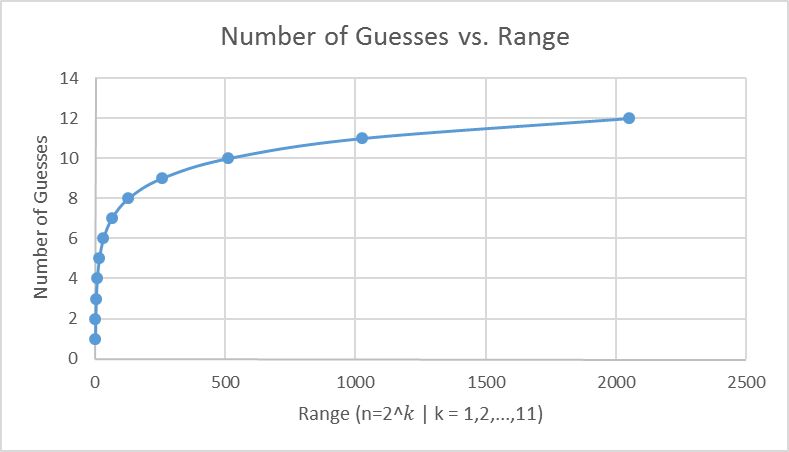
\includegraphics{pasted4}\newline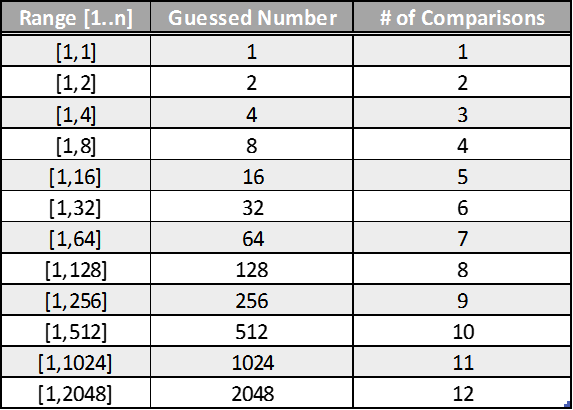
\includegraphics{pasted6}
\begin{enumerate}
\item Provide a mathematical formula/function which takes $n$ as an argument,
where $n$ is equal to the upper value of the testing ranges, and
returns as its value the maximum number of questions for the range
$[1,\dots,n]$. Does your formula match computed output for a given
input? Justify your answer.\textbf{}\\
\textbf{Formula: ${log}_{2}(n)+1$} No, the formula only outputs the
max number of guesses. Depending on the input and number, it takes
the algorithm different number of guesses every time.\end{enumerate}
\begin{lyxcode}
\textbf{
\includegraphics[scale=0.75]{pasted2}}\end{lyxcode}
\begin{enumerate}
\item How can you modify your formula/function if the number to be guessed
is between $1$ and $N$, where $N$ is not an exact power of two?
Test your program using input in ranges starting from $1$ to $2^{k}-1,\,\,k=2,3,\dots11.$


\textbf{Modified Formula:$\lfloor({log}_{2}(N))+1\rfloor$}

\end{enumerate}


\includegraphics[scale=0.75]{pasted3}

\item Use Big-O asymptotic notation to classify this algorithm.
\end{enumerate}

O(${log}_{2}(n)$)


Submit for grading an electronic copy of your code and solutions to
the questions above. 


\medskip{}



\title{Points Distribution}


(a) (b)\textbf{ }\textcolor{red}{(5 pts)}\uline{ \# guesses in
a table}; \textcolor{red}{(5 pts)}\uline{ A plot in the report;
}\textcolor{red}{(15 pts)} \uline{Program code using STL vector
and exception}


(c)\textcolor{red}{{} (5 pts)}\uline{ A math formula of n;} \textcolor{red}{(5
pts)} \uline{Formula results compared to \# guesses}


(d)\textcolor{red}{{} (5 pts)}\uline{ A math formula of N; }\textcolor{red}{(5
pts)}\uline{ Program code (and the second table)}


(e) \textcolor{red}{(5 pts)}\uline{ A big-O function}


Submit an electronic copy of your code and results of all your experiments
for grading.


\newpage{}

\item (15 points) Write a C++ function using the STL string which can determine
if a string $s$ is a palindrome, that is, it is equal to its reverse.
For example, ``racecar'' and ``gohangasalamiimalasagnahog'' are
palindromes. Provide 7 test cases, including: the empty string, 4
string which are palindromes and two string which are not palindromes.
Write the running time function in terms of $n$, the length of the
string, and its big-O notation to represent the efficiency of your
algorithm. Submit an electronic copy of your code and results of all
your experiments for grading.\newline\newline %
\begin{minipage}[t]{1\columnwidth}%
The running time of the is\_palindrome is f(n) = 3(n/2)+3 which is
O(n)%
\end{minipage}\lstinputlisting{2.cpp}
\item (10 points) Write a function (in pseudo code) which takes as an input
an object of \texttt{vector} type and removes an element at the rank
\texttt{k }in the constant time, O(1). Assume that the order of elements
does not matter.\newline\newline %
\begin{minipage}[t]{1\columnwidth}%
\textbf{Algorithm} remove\_at\_rank(Vector V, integer k)

\textbf{\qquad{}Input}: vector and index of element that is to be
removed

\textbf{\qquad{}Output}: vector that has element k removed

//switch back element with element at k

t$\leftarrow$V{[}k{]}

V{[}k{]}$\leftarrow$V{[}size-1{]}

V{[}size-1{]}$\leftarrow$t

remove back element\qquad{} //which is now V{[}k{]}%
\end{minipage}
\item (10 points) \textbf{(R-4.39 p. 188)} Al and Bob are arguing about
their algorithms. Al claims his $O(n$log$n)$- time method is always
faster than Bob's O$(n^{2})$- time method. To settle the issue, they
perform a set of experiments. To Al's dismay, they find that if $n<100$,
the O$(n^{2})$-time algorithm runs faster, and only when $n\geq100$
is the O$(n$log$n)$-time one better. Explain how this is possible.
\newline\\
\begin{minipage}[t]{1\columnwidth}%
If you were to examine the graph of n\textsuperscript{2}and nlog(n)
you would see that they would intersect around n = 100. Also, you
would see that for n < 100, n\textsuperscript{2}is in fact below
nlog(n). Another way to explain it is through a direct proof. Take
n to be 99. Then n\textsuperscript{2}= 9801 and nlog(n) = 9872.306
which would means Bob's algorithm is faster then Al's when n = 99.
\newline%
\end{minipage}
\item (15 points) Find the running time functions and classify the algorithms
using Big-O asymptotic notation presented in the exercise 4.4, p.
187.

\begin{lyxcode}


\textbf{Algorithm}~Ex1(A):~\\
~~\textbf{Input}:~An~array~A~storing~$n\geq1$~integers.~\\
~~\textbf{Output}:~The~sum~of~the~elements~at~even~cells~in~A.~\\
$s\leftarrow A[0]$~\\
\textbf{for}~$i\leftarrow2$~\textbf{to}~$n-1$~\textbf{by~}increments~of~2\textbf{~do}~\\
~~~$s\leftarrow s+A[i]$~\\
\textbf{return}~s\newline%
\begin{minipage}[t]{1\columnwidth}%
f(n) = $2(\frac{(n-2)}{2})$+1 = n-1 = O(n)\newline\newline%
\end{minipage}

\textbf{Algorithm}~Ex2(A):~\\
~~~\textbf{Input}:~An~array~A~storing~$n\geq1$~integers.~\\
~~~\textbf{Output}:~The~sum~of~the~prefix~sums~in~A.~\\
$s\leftarrow0$~\\
\textbf{for}~i~$\leftarrow$0~\textbf{to}~$n-1$~\textbf{do}~\\
~~~$s\leftarrow s+A[0]$~\\
~~~\textbf{for}~$j\leftarrow1$~\textbf{to}~$n$~\textbf{do}~\\
~~~~~~$s\leftarrow s+A[j]$~\\
\textbf{return}~s\newline%
\begin{minipage}[t]{1\columnwidth}%
f(n) = 2n(2n) + 1 = 4n\textsuperscript{2}+1 = O(n\textsuperscript{2})
\newline\newline%
\end{minipage}

\textbf{Algorithm}~Ex2(A):~\\
~~~\textbf{Input}:~An~array~A~storing~$n\geq1$~integers.~\\
~~~\textbf{Output}:~The~sum~of~the~prefix~sums~in~A.~\\
$s\leftarrow0$~\\
\textbf{for}~i~$\leftarrow$0~\textbf{to}~$n-1$~\textbf{do}~\\
~~~$s\leftarrow s+A[0]$~\\
~~~\textbf{for}~$j\leftarrow1$~\textbf{to}~$i$~\textbf{do}~\\
~~~~~~$s\leftarrow s+A[j]$~\\
\textbf{return}~s\newline%
\begin{minipage}[t]{1\columnwidth}%
f(n) = 2n + n($\frac{2(1-2^{n-1})}{1-2}$) = 2n + 2\textsuperscript{n}n
- 2n = O(n2\textsuperscript{n})%
\end{minipage}\vfill{}


\end{lyxcode}
\end{enumerate}

\end{document}
